% =====================================================================
%  SIH26242 - DakshSetu - Technical Report
%  Standalone technical documentation for the whole project.
%  Compile with: tectonic -X compile technical-report.tex
% =====================================================================
\documentclass[11pt,a4paper]{article}

\usepackage[T1]{fontenc}
\usepackage[utf8]{inputenc}
\usepackage{lmodern}
\usepackage{underscore}          % allow _ in text without escaping
\usepackage[a4paper,margin=2.05cm]{geometry}
\usepackage{amsmath}
\usepackage{array}
\usepackage{booktabs}
\usepackage{longtable}
\usepackage{tabularx}
\usepackage{enumitem}
\usepackage{xcolor}
\usepackage{titlesec}
\usepackage{fancyhdr}
\usepackage{tikz}
\usetikzlibrary{arrows.meta,positioning,shapes.geometric,fit,backgrounds}
\definecolor{navy}{HTML}{1F3864}
\definecolor{navyurl}{HTML}{1B4F9C}
\definecolor{soft}{HTML}{F2F5FA}
\definecolor{line}{HTML}{C9D4E6}
\definecolor{okgreen}{HTML}{1E7B4D}
\definecolor{warnred}{HTML}{B03A2E}
\usepackage[colorlinks=true,linkcolor=navyurl,citecolor=navyurl,urlcolor=navyurl]{hyperref}

\titleformat{\section}{\color{navy}\Large\bfseries}{\thesection}{0.6em}{}
\titleformat{\subsection}{\color{navy}\large\bfseries}{\thesubsection}{0.5em}{}
\titleformat{\subsubsection}{\color{navy}\normalsize\bfseries}{\thesubsubsection}{0.5em}{}
\titlespacing*{\section}{0pt}{1.4em}{0.5em}

\pagestyle{fancy}
\fancyhf{}
\fancyhead[L]{\small\color{navy}\textbf{DakshSetu} \textnormal{| SIH26242 Technical Report}}
\fancyfoot[C]{\small\thepage}
\renewcommand{\headrulewidth}{0.4pt}

\newcommand{\code}[1]{\texttt{\small #1}}
\newcommand{\status}[1]{\textcolor{navy}{\textbf{#1}}}
\newcolumntype{L}[1]{>{\raggedright\arraybackslash}p{#1}}

\setlist[itemize]{topsep=2pt,itemsep=1.5pt,parsep=0pt}
\setlist[enumerate]{topsep=2pt,itemsep=1.5pt,parsep=0pt}
\setlength{\emergencystretch}{3em}

\begin{document}

% ---------------------------------------------------------------- title
\begin{titlepage}
\centering
\vspace*{2.2cm}
{\color{navy}\rule{\textwidth}{1.4pt}}\\[0.6em]
{\Huge\bfseries\color{navy} DakshSetu}\\[0.35em]
{\large AI-Assisted Skill Assessment for Recognition of Prior Learning}\\[0.35em]
{\large\itshape Technical Report}\\[0.7em]
{\color{navy}\rule{\textwidth}{1.4pt}}\\[2.2em]

\begin{tabular}{L{4.2cm}L{9.5cm}}
\textbf{Programme} & Smart India Hackathon 2026 \\[2pt]
\textbf{Problem statement} & SIH26242 --- AI-Assisted Skill Assessment Tool for Recognition of Prior Learning (RPL) \\[2pt]
\textbf{Product} & DakshSetu (worker PWA + assessor portal + certification) \\[2pt]
\textbf{Repository} & \code{sih26242-rpl} --- npm-workspaces monorepo \\[2pt]
\textbf{Deliverable} & Web platform: contract-first API, offline-first PWA, AI-assisted scoring, verifiable certification \\[2pt]
\textbf{Version} & 1.0 \\[2pt]
\textbf{Date} & 2026 \\
\end{tabular}

\vfill
{\small This report documents the architecture, domain model, assessment
pipeline, security model, testing evidence, and operations of the
DakshSetu platform. All figures are taken from the working repository.}
\vspace{1.2cm}
\end{titlepage}

% ---------------------------------------------------------------- abstract
\section*{Executive summary}
\addcontentsline{toc}{section}{Executive summary}
Recognition of Prior Learning (RPL) lets experienced workers obtain formal
NSQF-aligned certification for skills already acquired on the job, without
retraining from scratch. The bottleneck is assessment: a fair, consistent,
auditable and low-cost way to judge a worker's competence. DakshSetu is an
end-to-end platform that runs a worker from self-declaration, through
AI-assisted trade mapping and a personalised practical plan, to evidence
capture, AI-assisted scoring, human assessment, and an instantly verifiable
digital certificate.

The system is built contract-first: a single TypeScript package
(\code{@sih/contracts}) defines every Zod schema, the assessment state
machine, and the complete HTTP route table (43 endpoints) from which the
OpenAPI document, the backend request validation, and the frontend typed
client are all derived. The backend is a layered Express~5 / MongoDB service
with pluggable drivers for AI, storage, upload and queueing; the frontend is
a React 18 PWA that works offline. The scoring engine is
\emph{deterministic-first}: objective items are auto-scored, AI is used only
where it adds value, and a human assessor always retains precedence. Critical
safety competencies act as a veto. Certificates carry a QR-linked public
verifier and a SHA-256 evidence/audit hash chain. The backend is covered by
124 automated tests across 14 suites; the full lifecycle was additionally
exercised end-to-end through the UI.

% ---------------------------------------------------------------- TOC
{\small\tableofcontents}
\newpage

% ================================================================ 1
\section{Introduction}
\subsection{Context}
Skill India's RPL track certifies workers against National Skills
Qualification Framework (NSQF) Qualification Packs (QPs) defined by sector
skill councils. A worker with ten years of site experience may have no paper
credential; conversely, a certificate should mean the holder can actually do
the job. Traditional assessor-led RPL is expensive, geographically
constrained, and can vary between assessors. Digital assessment can scale it,
but naive automation risks unfair or unexplainable outcomes --- particularly
on safety-critical competencies.

\subsection{Problem statement (SIH26242)}
Build an AI-assisted skill assessment tool for RPL that:
\begin{itemize}
\item lets workers self-declare experience, then maps them to the most
      suitable NSQF Qualification Pack;
\item generates a personalised, evidence-based assessment plan;
\item captures practical evidence (photos, video, narration) with
      integrity signals;
\item uses AI to assist scoring while keeping decisions explainable,
      fair and human-controlled;
\item issues a tamper-evident, publicly verifiable certificate.
\end{itemize}

\subsection{Design principles}
\begin{enumerate}
\item \textbf{Contract-first.} One source of truth for schemas, routes and
      the state machine; generated OpenAPI; no hand-written duplicate types.
\item \textbf{Deterministic-first AI.} Objective questions are auto-scored
      exactly; AI augments subjective items and never silently overrides a
      human.
\item \textbf{Safety as a veto.} Missing a critical-safety competency cannot
      be averaged away.
\item \textbf{Offline-first.} Low-connectivity worksites are the norm; the
      PWA queues work and reconciles later.
\item \textbf{Auditable by construction.} Every transition is recorded on a
      hash-chained audit log; evidence bytes are hashed.
\item \textbf{Trilingual.} English, Hindi and Marathi across the UI, tasks
      and narration.
\end{enumerate}

% ================================================================ 2
\section{Solution overview}
DakshSetu is a monorepo of three npm workspaces:

\begin{center}
\begin{tabular}{L{3.4cm}L{12.2cm}}
\toprule
\textbf{Workspace} & \textbf{Responsibility} \\
\midrule
\code{@sih/contracts} & Zod entities and API schemas, the assessment state
machine, route table, trade-pack schema, generated OpenAPI. \\[2pt]
\code{@sih/backend} & Express 5 API, MongoDB persistence, auth, evidence
storage (tus), AI/vision/ASR adapters, scoring, review, certification,
queue worker, realtime. \\[2pt]
\code{@sih/frontend} & \textbf{DakshSetu} React PWA: worker portal, assessor
portal, public verifier. \\
\bottomrule
\end{tabular}
\end{center}

\noindent A worker's journey is a linear, resumable state machine that can
loop once for reassessment:

\begin{center}
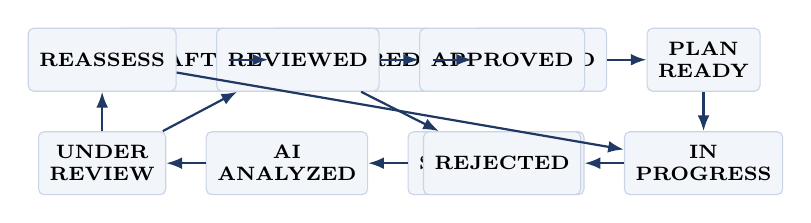
\begin{tikzpicture}[
  node distance=5mm and 5mm,
  box/.style={draw=line,fill=soft,rounded corners=2pt,align=center,
              font=\scriptsize\bfseries,inner sep=4pt,minimum height=8mm},
  arr/.style={-{Latex[length=2mm]},draw=navy,thick}]
\node[box] (a) {DRAFT};
\node[box,right=of a] (b) {DECLARED};
\node[box,right=of b] (c) {MAPPED};
\node[box,right=of c] (d) {PLAN\\READY};
\node[box,below=of d] (e) {IN\\PROGRESS};
\node[box,left=of e] (f) {SUBMITTED};
\node[box,left=of f] (g) {AI\\ANALYZED};
\node[box,left=of g] (h) {UNDER\\REVIEW};
\node[box,above=of h] (i) {REASSESS};
\node[box,right=of i] (j) {REVIEWED};
\node[box,right=of j] (k) {APPROVED};
\node[box,below=of k] (l) {REJECTED};
\draw[arr] (a)--(b); \draw[arr] (b)--(c); \draw[arr] (c)--(d); \draw[arr] (d)--(e);
\draw[arr] (e)--(f); \draw[arr] (f)--(g); \draw[arr] (g)--(h);
\draw[arr] (h)--(i); \draw[arr] (i)--(e);
\draw[arr] (h)--(j); \draw[arr] (j)--(k); \draw[arr] (j)--(l);
\end{tikzpicture}
\end{center}

% ================================================================ 3
\section{Architecture}
\subsection{Layers}
The backend follows a strict layering so that business logic is testable
without HTTP and HTTP concerns never leak into domain code:
\begin{itemize}
\item \textbf{Routes / handlers} (\code{src/routes/handlers}) --- thin; parse
      with contract schemas, call a service, shape the response.
\item \textbf{Services} (\code{src/services}) --- domain logic: assessment
      lifecycle, mapping, planning, analysis, scoring, review, certification,
      fairness, search, sync.
\item \textbf{Models} (\code{src/models}) --- Mongoose documents mirroring
      the contract entities.
\item \textbf{Drivers / adapters} --- AI (\code{ai/*}), storage
      (\code{storage/*}), upload (tus), OTP, queue. Selected by environment,
      so development runs fully keyless.
\item \textbf{Worker} (\code{src/worker}) --- a BullMQ consumer process; in
      the default inline mode the pipeline runs in-process.
\item \textbf{Realtime} --- Socket.IO pushes pipeline status to the client.
\end{itemize}

\subsection{Runtime topology}
\begin{itemize}
\item \textbf{API} --- Express 5 on Node $\ge$ 20, port 4000.
\item \textbf{Database} --- MongoDB 7 via Mongoose 9. Local dev can use an
      in-memory MongoDB (\code{mongodb-memory-server}) with \code{npm run
      dev:local}, requiring no Docker.
\item \textbf{Redis 7 + BullMQ} --- optional; when \code{REDIS_URL} is unset
      the queue driver falls back to \code{inline}.
\item \textbf{Storage} --- \code{local} filesystem or S3-compatible
      (\code{s3}, e.g.\ Cloudflare R2).
\item \textbf{Frontend} --- Vite 5 SPA served statically, installable as a
      PWA.
\end{itemize}

% ================================================================ 4
\section{Contract-first design}
\code{@sih/contracts} is the spine of the system.

\subsection{Entities and schemas (Zod)}
Every entity --- Assessment, Declaration, QPMatch, AssessmentPlan, PublicTask,
TaskResponse, Evidence, AIAnalysis, AssessorReview, Decision, CompetencyReport,
Certificate, AuditLogEntry, WorkerProfile, User, TradePack --- is a Zod schema
with inferred TypeScript types. The same schemas validate backend input, type
the frontend, and generate documentation. Zod~4 is used throughout.

\subsection{The route table}
The full HTTP surface is a single array of route descriptors (43 routes),
each carrying method, path, tag, summary, auth role, params, query, body and
response schema. Consequences:
\begin{itemize}
\item the backend \emph{throws at boot} if any declared route lacks a handler
      (or a handler exists that is not declared) --- the contract and the
      implementation cannot silently drift;
\item the OpenAPI document is generated from the same table
      (\code{npm run openapi} writes the \code{openapi.json} document);
\item auth middleware derives required roles from the table, not from
      scattered per-route decorations.
\end{itemize}

\subsection{State machine as a contract}
\code{ASSESSMENT_TRANSITIONS} is the authority for allowed status changes.
The backend rejects illegal transitions; the frontend imports the same table
(via \code{canTransition}) to render optimistic UI. The 12 statuses are shown
in Appendix~B.

% ================================================================ 5
\section{Domain model and lifecycle}
\subsection{Roles}
Four roles: \status{worker}, \status{assessor},
\status{authorized_assessor}, \status{admin}. A worker authenticates by phone
OTP; assessors by email and password (bcrypt). Only an authorised assessor may
record the final decision.

\subsection{Entities}
\begin{itemize}
\item \textbf{WorkerProfile} --- demographics, trades, versioned for
      last-write-wins sync.
\item \textbf{Declaration} --- years of experience, work types, tools, tasks,
      sectors, employment types (free labels + free text).
\item \textbf{QPMatch} --- ranked NSQF qualification-pack candidates with a
      confidence and the signals that produced it.
\item \textbf{AssessmentPlan} --- an ordered list of \emph{PublicTask}s with
      rubric weights summing to 100\,\%.
\item \textbf{TaskResponse} --- the worker's answer to one task; auto-scored
      where objective.
\item \textbf{Evidence} --- a media artefact (photo/video/audio/document)
      with a content hash, GPS, device and capture metadata.
\item \textbf{AIAnalysis} --- per-task AI result: score, confidence, routing
      and flags.
\item \textbf{AssessorReview} --- per-task final scores (accept or override),
      comments, outcome.
\item \textbf{Decision} --- APPROVED/REJECTED by an authorised assessor.
\item \textbf{CompetencyReport} --- NSQF result: overall score, NOS-wise
      results, recommendation, critical-safety pass, suggested NSQF level.
\item \textbf{Certificate} --- number, holder, QP, level, score, QR, and a
      revocation flag.
\item \textbf{AuditLogEntry} --- hash-chained record of every event.
\end{itemize}

\subsection{Task types}
Six task types drive the runner and the analysis adapters:
\begin{center}
\begin{tabular}{L{4.1cm}L{11.5cm}}
\toprule
\textbf{Type} & \textbf{Purpose / scoring} \\
\midrule
\code{mcq} & Multiple-choice knowledge check; deterministic auto-score. \\
\code{tool_identification} & Identify correct tools/instruments from an
  image set; deterministic. \\
\code{checklist} & Ordered/compound procedural checks; item-weighted. \\
\code{practical_photo} & Geotagged still evidence (min/max count) assessed
  by the vision adapter. \\
\code{practical_video} & Video evidence; keyframe + (optional) ASR analysis. \\
\code{narration} & Spoken explanation; ASR transcript confirmed by the
  worker, assessed by the LLM. \\
\bottomrule
\end{tabular}
\end{center}

% ================================================================ 6
\section{Assessment pipeline}
\subsection{Declaration and mapping}
The worker submits a self-declaration. The mapping service combines
deterministic keyword/NOS matching (using trade-pack aliases) with an optional
embedding pass, and returns the top-3 QPs with confidence and signal
explanations. The worker confirms a trade, moving the assessment to
\status{MAPPED}.

\subsection{Plan generation}
For the chosen trade pack the planner instantiates tasks from
\emph{taskBlueprints} and MCQs from the pack's MCQ bank, attaches rubric
weights (normalised to 100\,\%), evidence specifications (media kinds,
min/max counts, GPS and narration requirements) and NOS references. The plan
is stored and the assessment becomes \status{PLAN\_READY}.

\subsection{Task runner and evidence capture}
Answers are submitted per task and auto-scored where objective. Evidence is
uploaded with \emph{tus} (resumable, \code{@tus/server} + file store) and
registered as metadata; the backend verifies the content hash on finalisation.
GPS and a worker-in-frame cue support practical authenticity.

\subsection{AI analysis}
On \code{POST /submit} the assessment becomes \status{SUBMITTED} and the
analysis pipeline is queued. The pipeline is modular:
\begin{itemize}
\item \textbf{Deterministic} scoring runs for objective items with no model
      call.
\item \textbf{LLM} adapter scores narration and rubric judgements.
\item \textbf{Vision} adapter assesses photos (tool identification, safety
      practice visible in frame).
\item \textbf{ASR} adapter transcribes narration/audio;
      \code{ffmpeg} extracts video keyframes.
\end{itemize}
Each result carries a confidence; items below
\code{AI_CONFIDENCE_HUMAN_ROUTE} (default 0.65) are routed to a human.
Critical-safety items raise flags. When finished the assessment is
\status{AI\_ANALYZED}. Modes: \code{AI_MODE=mock} (keyless, deterministic ---
used in dev and tests) or \code{auto} with OpenAI-compatible endpoints.

\subsection{Scoring engine}
The score is computed by \code{scoring.service}:
\begin{itemize}
\item the \textbf{assessor's final score takes precedence} over the AI score
      (review-over-AI);
\item per-task weighted aggregation to an overall score out of 100;
\item \textbf{NOS-wise} roll-ups feed the competency report;
\item a \textbf{critical-safety veto}: any unmet critical-safety competency
      fails the safety gate regardless of the average;
\item NSQF level banding yields a suggested level;
\item the recommendation is one of \code{certify},
      \code{certify_with_bridge}, \code{reassess}, \code{not_certified}.
\end{itemize}

\subsection{Review and decision}
An assessor claims the case from the shared queue
(\status{AI\_ANALYZED} $\rightarrow$ \status{UNDER\_REVIEW}); the queue is
ordered oldest-first for fairness, and claiming is exclusive. The assessor
reviews each task side by side with the deterministic and AI scores, flags and
routing, accepting or overriding, then submits an outcome of \status{REVIEWED}
or \status{REASSESS} (the latter returns the assessment to
\status{IN\_PROGRESS} for the round). An \status{authorized_assessor} records
the final \status{APPROVED} or \status{REJECTED} decision; the competency
report is generated and, on approval, a certificate is issued.

\subsection{Report, certificate and verification}
The competency report presents the overall score, NOS-wise results,
consistency, assessor overrides, critical-safety status and suggested NSQF
level. On approval a certificate is minted
(\code{SIH-RPL-<year>-XXXXXXXX}) and rendered to PDF with \code{pdfkit}, with
a QR code (\code{qrcode}) pointing at the public verifier
\code{/verify/<certificateNo>}. The verifier is unauthenticated and returns
validity, holder, trade, level, score and issue date. Revocation is supported
via a flag on the certificate.

% ================================================================ 7
\section{Offline-first and synchronisation}
Worksites frequently lack connectivity, so the PWA is offline-capable:
\begin{itemize}
\item an \textbf{IndexedDB outbox} queues profile, declaration and answer
      operations; conflicting writes use last-write-wins with a client
      timestamp;
\item every mutating request carries an \textbf{Idempotency-Key} so retries
      after reconnection cannot double-apply;
\item a \textbf{sync push/pull} API reconciles the outbox with a cursor-based
      pull of server changes;
\item uploads are \textbf{resumable} (tus), so an interrupted photo/video
      upload continues rather than restarting;
\item a service worker precaches the app shell and applies
      stale-while-revalidate to contract GETs.
\end{itemize}

% ================================================================ 8
\section{Security, privacy and integrity}
\begin{itemize}
\item \textbf{Authentication} --- short-lived JWT access tokens (default 30
      min) with rotating refresh tokens (default 30 days, revocable);
      bcrypt for assessor passwords; phone OTP for workers with mock,
      Firebase or MSG91 providers.
\item \textbf{Authorisation} --- role checks derived from the route table;
      every assessment read is scoped to its owner or an assessor role.
\item \textbf{Hardening} --- Helmet, CORS allow-list, request size limits,
      and schema validation of all bodies/params/query.
\item \textbf{Evidence integrity} --- content is hashed (SHA-256); the audit
      log chains each entry to the previous hash, so tampering is detectable.
\item \textbf{Privacy} --- evidence is served only to authorised principals;
      fairness analytics are aggregate and descriptive (no attribute is ever
      used in an automated decision).
\end{itemize}

% ================================================================ 9
\section{Fairness and multilingual support}
\subsection{Fairness}
Regional language, gender and region attributes are recorded to
\emph{monitor} outcomes, not to drive them. \code{GET
/api/v1/admin/fairness} reports approval rates and mean scores by dimension
so that bias in AI-assisted scoring can be detected and corrected; the API
and the UI both state explicitly that the analysis is descriptive only.

\subsection{Multilingual}
The UI, the assessment tasks and narration support English, Hindi and Marathi.
Narration is captured as audio and transcribed; the worker confirms the
transcript before it is scored, keeping the worker in control of what is
assessed. Trade packs provide bilingual titles and aliases.

% ================================================================ 10
\section{Frontend --- DakshSetu PWA}
\subsection{Stack}
React 18.3, React Router 6.28, TanStack Query 5.59 for server state, Vite 5.4
for build/HMR, and \code{vite-plugin-pwa} 0.20 (Workbox) for the manifest and
service worker. The design system is a small set of accessible components
(Card, Button, Field, Alert, StatusBadge, Stepper, \dots) using a
government-friendly navy/soft palette.

\subsection{Portals}
\begin{itemize}
\item \textbf{Worker} --- OTP login; dashboard of assessments; a
      declaration $\rightarrow$ map $\rightarrow$ plan wizard; the task
      runner (all six task types with evidence capture); the results screen
      with the NOS-wise report and certificate download.
\item \textbf{Assessor} --- queue; review screen with per-task AI vs
      deterministic scores, confidence, routing and safety flags; decision
      screen; fairness analytics.
\item \textbf{Public} --- the certificate verifier, reachable with no login.
\end{itemize}

\subsection{Realtime and resilience}
Socket.IO delivers pipeline status so the worker sees progress from submission
through analysis. The app is installed like a native app, works offline, and
resyncs automatically.

% ================================================================ 11
\section{Testing and verification}
\subsection{Automated suite}
The backend ships \textbf{124 tests across 14 suites} (Vitest + Supertest over
an in-memory MongoDB, \code{AI_MODE=mock}, inline queue). Suites cover auth,
assessments, declaration/mapping, planning, answers, evidence, analysis,
scoring, review, report/decision/certificate, sync, fairness, trade packs and
bilingual behaviour.

\subsection{End-to-end walkthrough}
The complete lifecycle was exercised through the running UI and API, not just
unit tests. A worker was created by phone OTP, declared experience, was mapped
to \emph{Electrician - Domestic Solutions} (NSQF~3), received a 37-task plan
with rubric weights summing to 100\,\%, completed all six task types, and
submitted. Inline analysis produced \status{AI\_ANALYZED}; an authorised
assessor claimed the case, reviewed it and recorded a decision; the report
listed NOS-wise results with a critical-safety veto; and the certificate's
number (\code{SIH-RPL-2026-9614F4F9}) verified as valid on the public
verifier, which returned the holder, trade, NSQF level and score. The audit
trail showed the full hash-chained history from creation to approval.

\subsection{Continuous checks}
TypeScript is strict across all three workspaces; the frontend build
(\code{tsc --noEmit \&\& vite build}) and the backend type-check run in CI-style
local commands. Because the contract throws at boot on a route/handler
mismatch, an integration failure surfaces immediately.

% ================================================================ 12
\section{Operations and deployment}
\subsection{Local development}
\begin{itemize}
\item \code{npm run dev:local} --- builds contracts, boots an in-memory
      MongoDB, and starts the API with keyless mock AI/OTP and the inline
      queue. No Docker required.
\item \code{npm run infra:up} --- Docker Compose with MongoDB~7 and
      Redis~7 (for the BullMQ driver).
\item \code{npm run dev:frontend} --- Vite dev server; \code{dev:worker} ---
      the BullMQ worker.
\end{itemize}

\subsection{Containers}
The \code{Dockerfile} is a multi-stage \code{node:20-alpine} build: install,
compile contracts then backend, and a runtime image that installs
\code{ffmpeg} (for video) and runs as a non-root user with a
\code{/health} healthcheck. \code{docker-compose.prod.yml} provides the
production topology.

\subsection{Configuration}
A single \code{.env} drives all drivers: database, queue, storage, auth,
OTP provider, and AI. Sensible defaults let the whole stack run keyless; real
credentials switch individual adapters to Firebase/MSG91, OpenAI-compatible
models, or S3/R2 storage without code changes. The public base URL and
certificate prefix are configurable for QR links.

% ================================================================ 13
\section{Trade pack catalogue}
Four NSQF qualification packs are implemented as versioned JSON, each aligned
to a real QP from a sector skill council, with NOS units, tools, safety
topics, an MCQ bank, task blueprints, thresholds and bridge-training
suggestions.

\begin{center}
\small
\begin{tabular}{L{2.4cm}L{2.2cm}L{3.6cm}L{1.1cm}L{1.1cm}L{1.2cm}L{1.9cm}}
\toprule
\textbf{Pack} & \textbf{QP ID} & \textbf{Council} & \textbf{NSQF} & \textbf{NOS} & \textbf{MCQ} & \textbf{Blueprints} \\
\midrule
Electrician & PSS/Q6001 & PSSC & 3 & 11 & 28 & 11 \\
Welder & CSC/Q0204 & CGSC & 3 & 5 & 24 & 10 \\
Plumber & PSC/Q0104 & WMPSC & 4 & 8 & 24 & 12 \\
Mason & CON/Q0103 & CSDCI & 3 & 8 & 24 & 12 \\
\bottomrule
\end{tabular}
\end{center}

\noindent\textbf{Electrician - Domestic Solutions} (PSS/Q6001, PSSC, NSQF~3) is
the flagship pack: house wiring, appliances, protective devices and safety,
with 22 tools, 16 safety topics and 5 sources of truth.

% ================================================================ 14
\section{API surface}
The API exposes 43 routes grouped by tag: \code{meta} (health),
\code{auth}, \code{profile}, \code{assessments}, \code{declaration},
\code{mapping}, \code{plan}, \code{evidence}, \code{analysis},
\code{review}, \code{report}, \code{sync}, \code{trades} and \code{admin}.
Worker routes require a worker token; assessor routes an assessor role; the
decision route specifically requires \code{authorized_assessor}; verification
and trade discovery are public. The complete route reference is in
Appendix~A and is generated from \code{contracts/openapi.json}.

% ================================================================ 15
\section{Limitations and future work}
\begin{itemize}
\item The AI adapters are keyless mocks in development; production accuracy
      depends on a configured model, and prompts/calibration should be
      validated per trade.
\item Video analysis uses keyframes and optional ASR rather than continuous
      pose/object tracking.
\item Certificates are PDF + QR with a server-side verifier; verifiable
      credentials (W3C VC) and a blockchain anchor are natural extensions.
\item Offline conflict resolution is last-write-wins; per-field merge with a
      CRDT for concurrent multi-device edits is future work.
\item Larger, psychometrically validated item banks and calibration of the
      confidence threshold are required before national rollout.
\end{itemize}

% ================================================================ appendix A
\newpage
\appendix
\section{API route reference}
\footnotesize
\begin{longtable}{L{1.15cm}L{7.7cm}L{1.95cm}L{4.5cm}}
\toprule
\textbf{Method} & \textbf{Path} & \textbf{Auth} & \textbf{Summary} \\
\midrule
\endfirsthead
\toprule
\textbf{Method} & \textbf{Path} & \textbf{Auth} & \textbf{Summary} \\
\midrule
\endhead
\bottomrule
\endlastfoot
GET & \code{/health} & public & Liveness + dependency checks \\
POST & \code{/api/v1/auth/otp/request} & public & Request phone OTP \\
POST & \code{/api/v1/auth/otp/verify} & public & Verify OTP, get session \\
POST & \code{/api/v1/auth/assessor/register} & public & Register assessor \\
POST & \code{/api/v1/auth/assessor/login} & public & Assessor login \\
POST & \code{/api/v1/auth/refresh} & public & Refresh tokens \\
POST & \code{/api/v1/auth/logout} & any & Revoke refresh token \\
GET & \code{/api/v1/auth/me} & any & Current user + profile \\
GET & \code{/api/v1/profile} & worker & Get own worker profile \\
PATCH & \code{/api/v1/profile} & worker & Update profile (LWW + version) \\
POST & \code{/api/v1/assessments} & worker & Create assessment (DRAFT) \\
GET & \code{/api/v1/assessments} & any & List assessments (role-scoped) \\
GET & \code{/api/v1/assessments/:id} & any & Get assessment + history \\
POST & \code{/api/v1/assessments/:id/declaration} & worker & Self-declaration (DECLARED) \\
GET & \code{/api/v1/assessments/:id/declaration} & any & Get declaration \\
POST & \code{/api/v1/assessments/:id/map} & worker & AI NSQF mapping (MAPPED) \\
GET & \code{/api/v1/assessments/:id/mapping} & any & Get QP match \\
POST & \code{/api/v1/assessments/:id/plan} & worker & Generate plan (PLAN\_READY) \\
GET & \code{/api/v1/assessments/:id/plan} & any & Get plan (keys stripped) \\
POST & \code{/api/v1/assessments/:id/start} & worker & Start / resume (IN\_PROGRESS) \\
POST & \code{/api/v1/assessments/:id/answers} & worker & Submit task answers \\
GET & \code{/api/v1/assessments/:id/answers} & any & List task responses \\
POST & \code{/api/v1/assessments/:id/submit} & worker & Submit (queues AI) \\
POST & \code{/api/v1/assessments/:id/evidence} & worker & Register evidence metadata \\
GET & \code{/api/v1/assessments/:id/evidence} & any & List evidence \\
GET & \code{/api/v1/evidence/:id/content} & any & Stream evidence bytes \\
GET & \code{/api/v1/assessments/:id/analysis} & any & Get AI analysis \\
GET & \code{/api/v1/assessments/:id/analysis/status} & any & Pipeline status \\
POST & \code{/api/v1/assessments/:id/review/claim} & assessor & Claim review \\
POST & \code{/api/v1/assessments/:id/review} & assessor & Submit review \\
GET & \code{/api/v1/assessments/:id/review} & any & Get latest review \\
GET & \code{/api/v1/assessor/queue} & assessor & Assessor queue \\
GET & \code{/api/v1/assessments/:id/report} & any & Competency report \\
POST & \code{/api/v1/assessments/:id/decision} & authorized\_assessor & Final decision \\
GET & \code{/api/v1/assessments/:id/decision} & any & Get decision \\
GET & \code{/api/v1/certificates/:id/pdf} & any & Certificate PDF (QR) \\
GET & \code{/api/v1/assessments/:id/audit} & assessor & Tamper-evident audit trail \\
GET & \code{/api/v1/verify/:certificateNo} & public & Public certificate verification \\
POST & \code{/api/v1/sync/push} & worker & Push offline ops (idempotent) \\
GET & \code{/api/v1/sync/pull} & worker & Pull changes since cursor \\
GET & \code{/api/v1/trades} & public & List trade packs \\
GET & \code{/api/v1/trades/:id} & public & Full trade pack (QP/NOS/rubric) \\
GET & \code{/api/v1/admin/fairness} & assessor & Fairness stats by dimension \\
\end{longtable}
\normalsize

% ================================================================ appendix B
\newpage
\section{State machine and task types}
\subsection{Statuses}
\begin{center}
\small
\begin{tabular}{L{3.4cm}L{11.5cm}}
\toprule
\textbf{Status} & \textbf{Meaning} \\
\midrule
DRAFT & Assessment created, nothing declared. \\
DECLARED & Self-declaration submitted. \\
MAPPED & A qualification pack has been confirmed. \\
PLAN\_READY & Personalised task plan generated. \\
IN\_PROGRESS & Worker is answering tasks / capturing evidence. \\
SUBMITTED & Answers submitted; AI pipeline queued. \\
AI\_ANALYZED & Automated analysis complete. \\
UNDER\_REVIEW & An assessor has claimed the case. \\
REASSESS & Assessor returned the case for another round. \\
REVIEWED & Review complete; awaiting final decision. \\
APPROVED & Authorised assessor approved; certificate issued. \\
REJECTED & Authorised assessor rejected. \\
\bottomrule
\end{tabular}
\end{center}

\subsection{Allowed transitions}
\begin{center}
\small
\begin{tabular}{L{3.4cm}L{11.5cm}}
\toprule
\textbf{From} & \textbf{Allowed to} \\
\midrule
DRAFT & DECLARED \\
DECLARED & MAPPED \\
MAPPED & PLAN\_READY \\
PLAN\_READY & IN\_PROGRESS \\
IN\_PROGRESS & SUBMITTED \\
SUBMITTED & AI\_ANALYZED \\
AI\_ANALYZED & UNDER\_REVIEW \\
UNDER\_REVIEW & REVIEWED, REASSESS \\
REASSESS & IN\_PROGRESS \\
REVIEWED & APPROVED, REJECTED \\
APPROVED & (terminal) \\
REJECTED & (terminal) \\
\bottomrule
\end{tabular}
\end{center}

\vfill
\begin{center}
{\color{navy}\rule{\textwidth}{0.8pt}}\\[0.4em]
{\small\color{navy}\textbf{DakshSetu} --- SIH26242 --- Technical Report --- 2026}
\end{center}

\end{document}
